\section{Comparativas}
Nuestro análisis de las heurísticas se centra en evaluar dos aspectos de las mismas: el tiempo requerido para ejecutarse y la cantidad promedio de conflictos que aparecen en la solución.


Nuestros test se basan en grafos generados de distintas maneras:

Por un lado generamos grafos completamente al azar, de los cuales no se conoce a priori si son coloreables o no (determinar si un grafo genérico tiene coloreo requiere un tiempo no polinomial, lo cual resulta impracticable para grafos grandes). Estos test, además de ser útiles para medir el tiempo de ejecución, también permiten analizar los resultados de las heurísticas de búsqueda local, ya que permiten detectar conflictos reportados por el goloso, que luego fueron corregidos por las otras heurísticas.

Por otro lado, para otros tests, utilizaremos grafos bipartitos completos, de los cuales tenemos la certeza de que son coloreables (ya que esta demostrado que todo grafo bipartito es coloreable utilizando dos colores). Estos grafos bipartitos se construyeron de manera que dos colores específicos están presentes como alternativas en todos los nodos,  y adicionalmente se agregaron otros colores elegidos al azar para cada nodo. De esta forma, se esta asegurando que existe al menos una solución de coloreo válida para todos los grafos bipartitos generados. Este coloreo consistiría en seleccionar el primer color que los nodos tienen en común para uno de los subconjuntos de vértices del grafo bipartito, y el otro color para el otro subconjunto.

Pensamos que los grafos bipartitos generados para los tests pueden resultar, aunque son un caso particular, pueden resultar interesantes para el análisis de la cantidad de conflictos de las heurísticas. Son grafos de los cuales se tiene la certeza de que son coloreables, pero que igualmente pueden contener una cantidad elevada de nodos y aristas.

A continuación se exponen los gráficos generados a partir de los resultados de los experimentos que ideamos e implementamos con el fin de hacer un análisis empirico del costo temporal y la calidad de los resultados obtenidos a partir del algoritmo goloso (Ejercicio 3) y de la vecindad 1 del algoritmo de búsqueda local (Ejercicio 4). 

Para ello, separamos este apartado en la observación de tres conjuntos de resultados:

\begin{itemize}
\item {Los obtenidos a partir de grafos completos}
\item {Los obtenidos a partir de grafos cíclicos}
\item {Los obtenidos a parir de grafos bipartitos completos}
\end{itemize}

Consideramos que hacerlo fue de especial relevancia, dado que al incrementar individualmente el valor de parámetros independientes es factible que se terminen realizando experimentos sobre grafos estructuralmente distintos, con poca o ninguna relación en cuanto a sus propiedades.\\
Los resultadoss se observan a continuación:\\


\subsection {Resultados obtenidos a partir de grafos cíclicos} 

En las figuras \ref{TiempoGreedyCiclico} y \ref{TiempoLocalCiclico} muestran los tiempos medidos observados para los dinstintos algoritmos en grafos cíclicos de distintos tamaños. \\
Observándolos en su conjunto, se puede apreciar que no sólo el algoritmo goloso se comporta de manera más uniforme en función de la entrada, si no que también se hace notorio que el mismo demanda un tiempo de cómputo mucho mayor en cada uno de los casos.\\  
 
\begin{figure}[H]
    \begin{center}
  	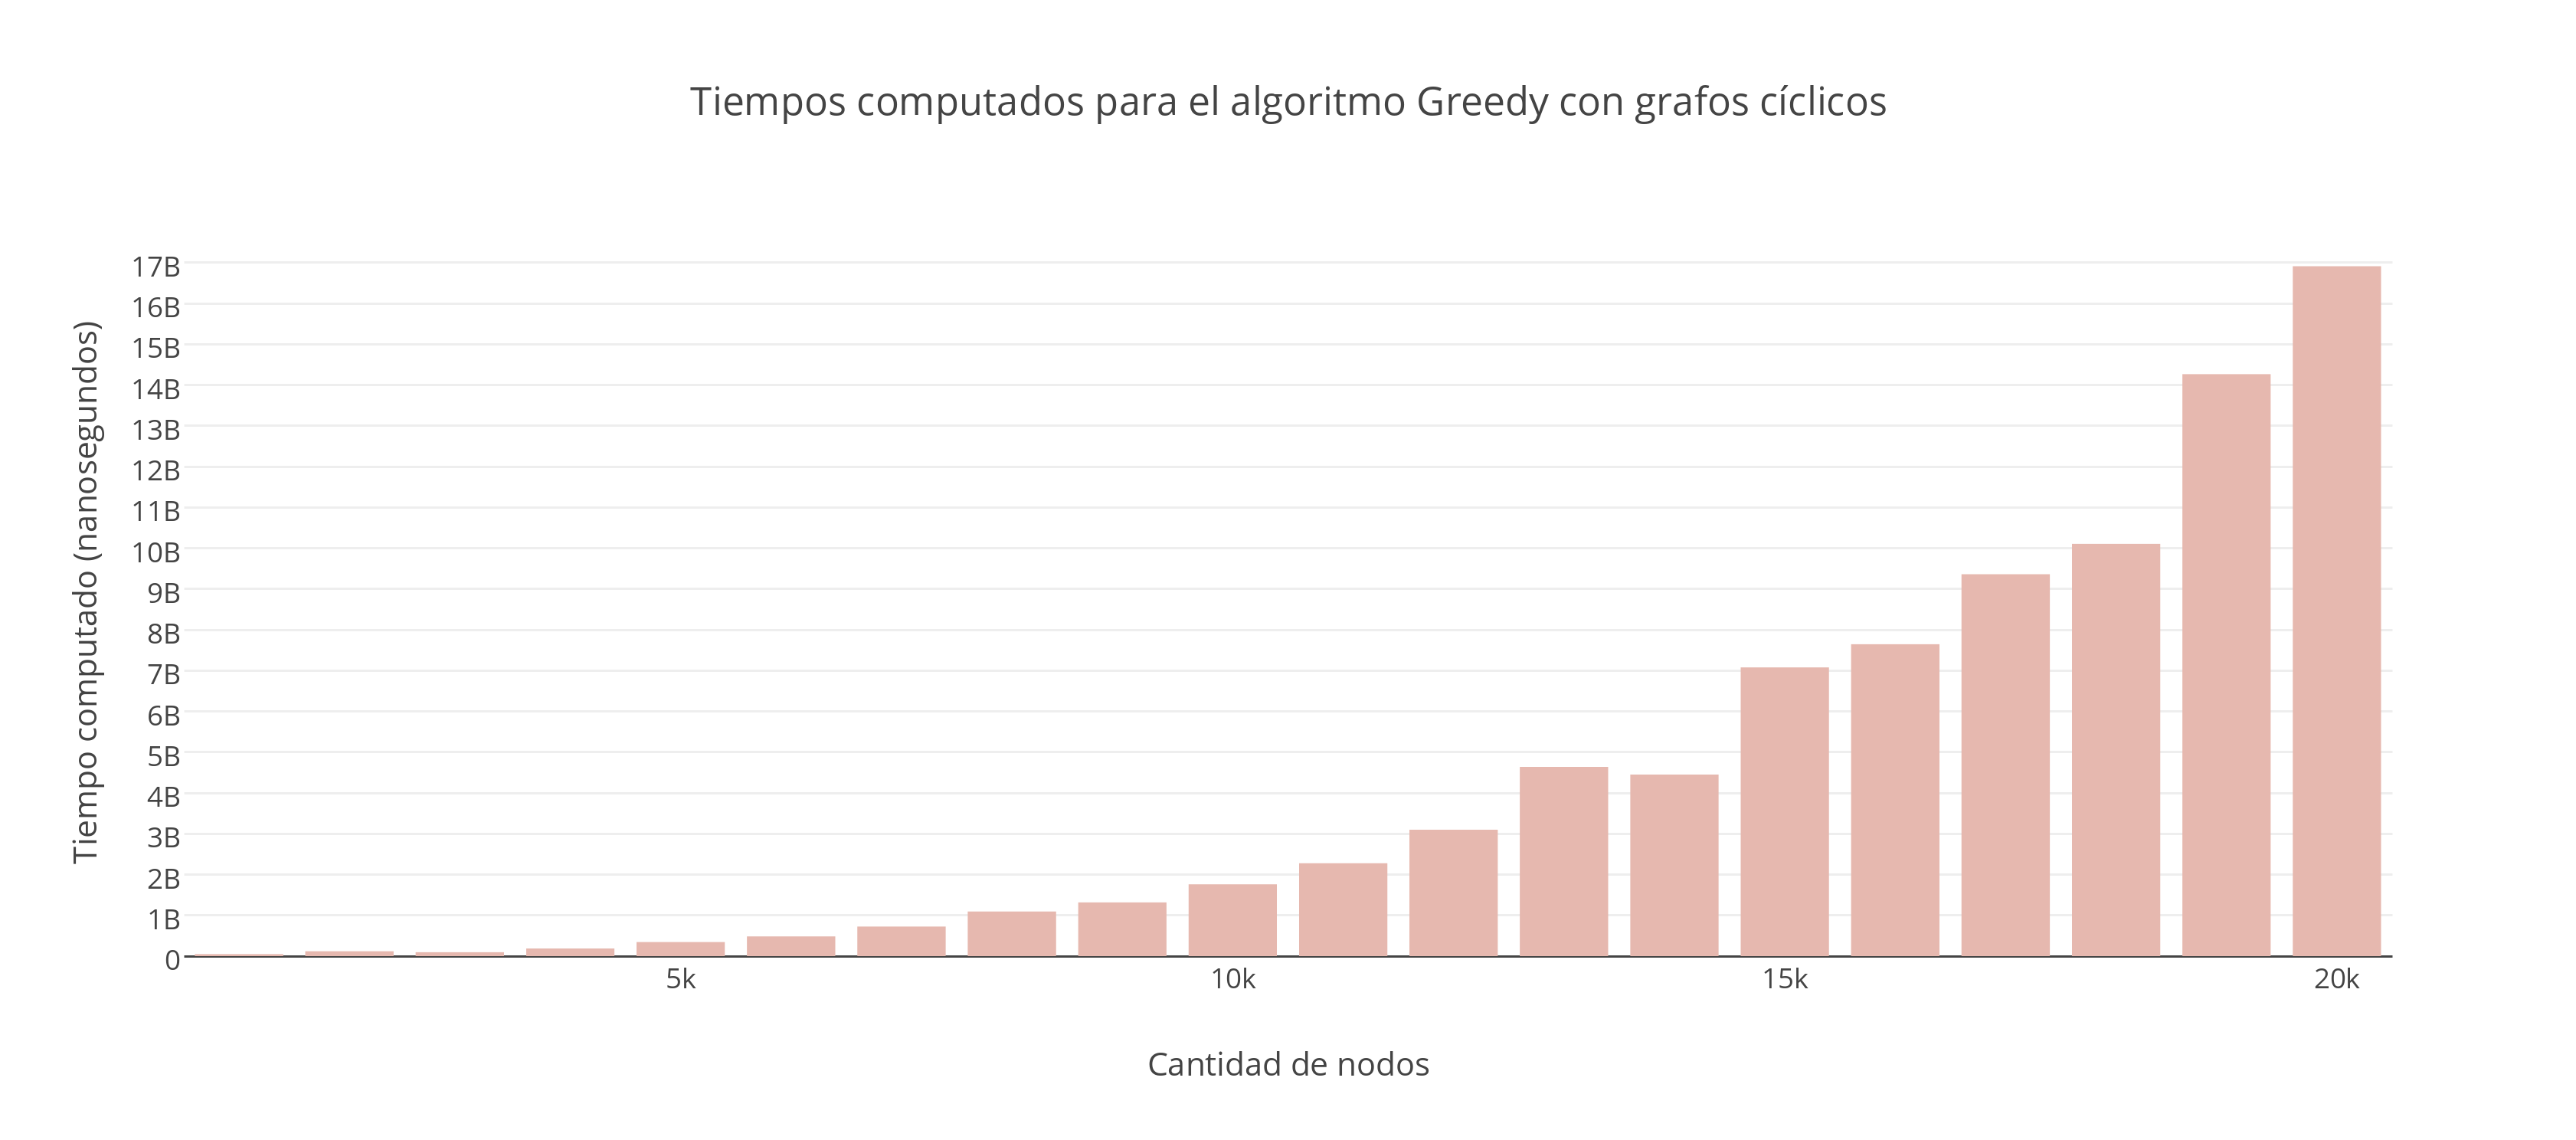
\includegraphics[width=18cm]{imagenes/Ej5/TiempoGreedyCiclico.png}
 	\label{TiempoGreedyCiclico}
    \end{center}
  \end{figure}

 \begin{figure}[H]
    \begin{center}
  	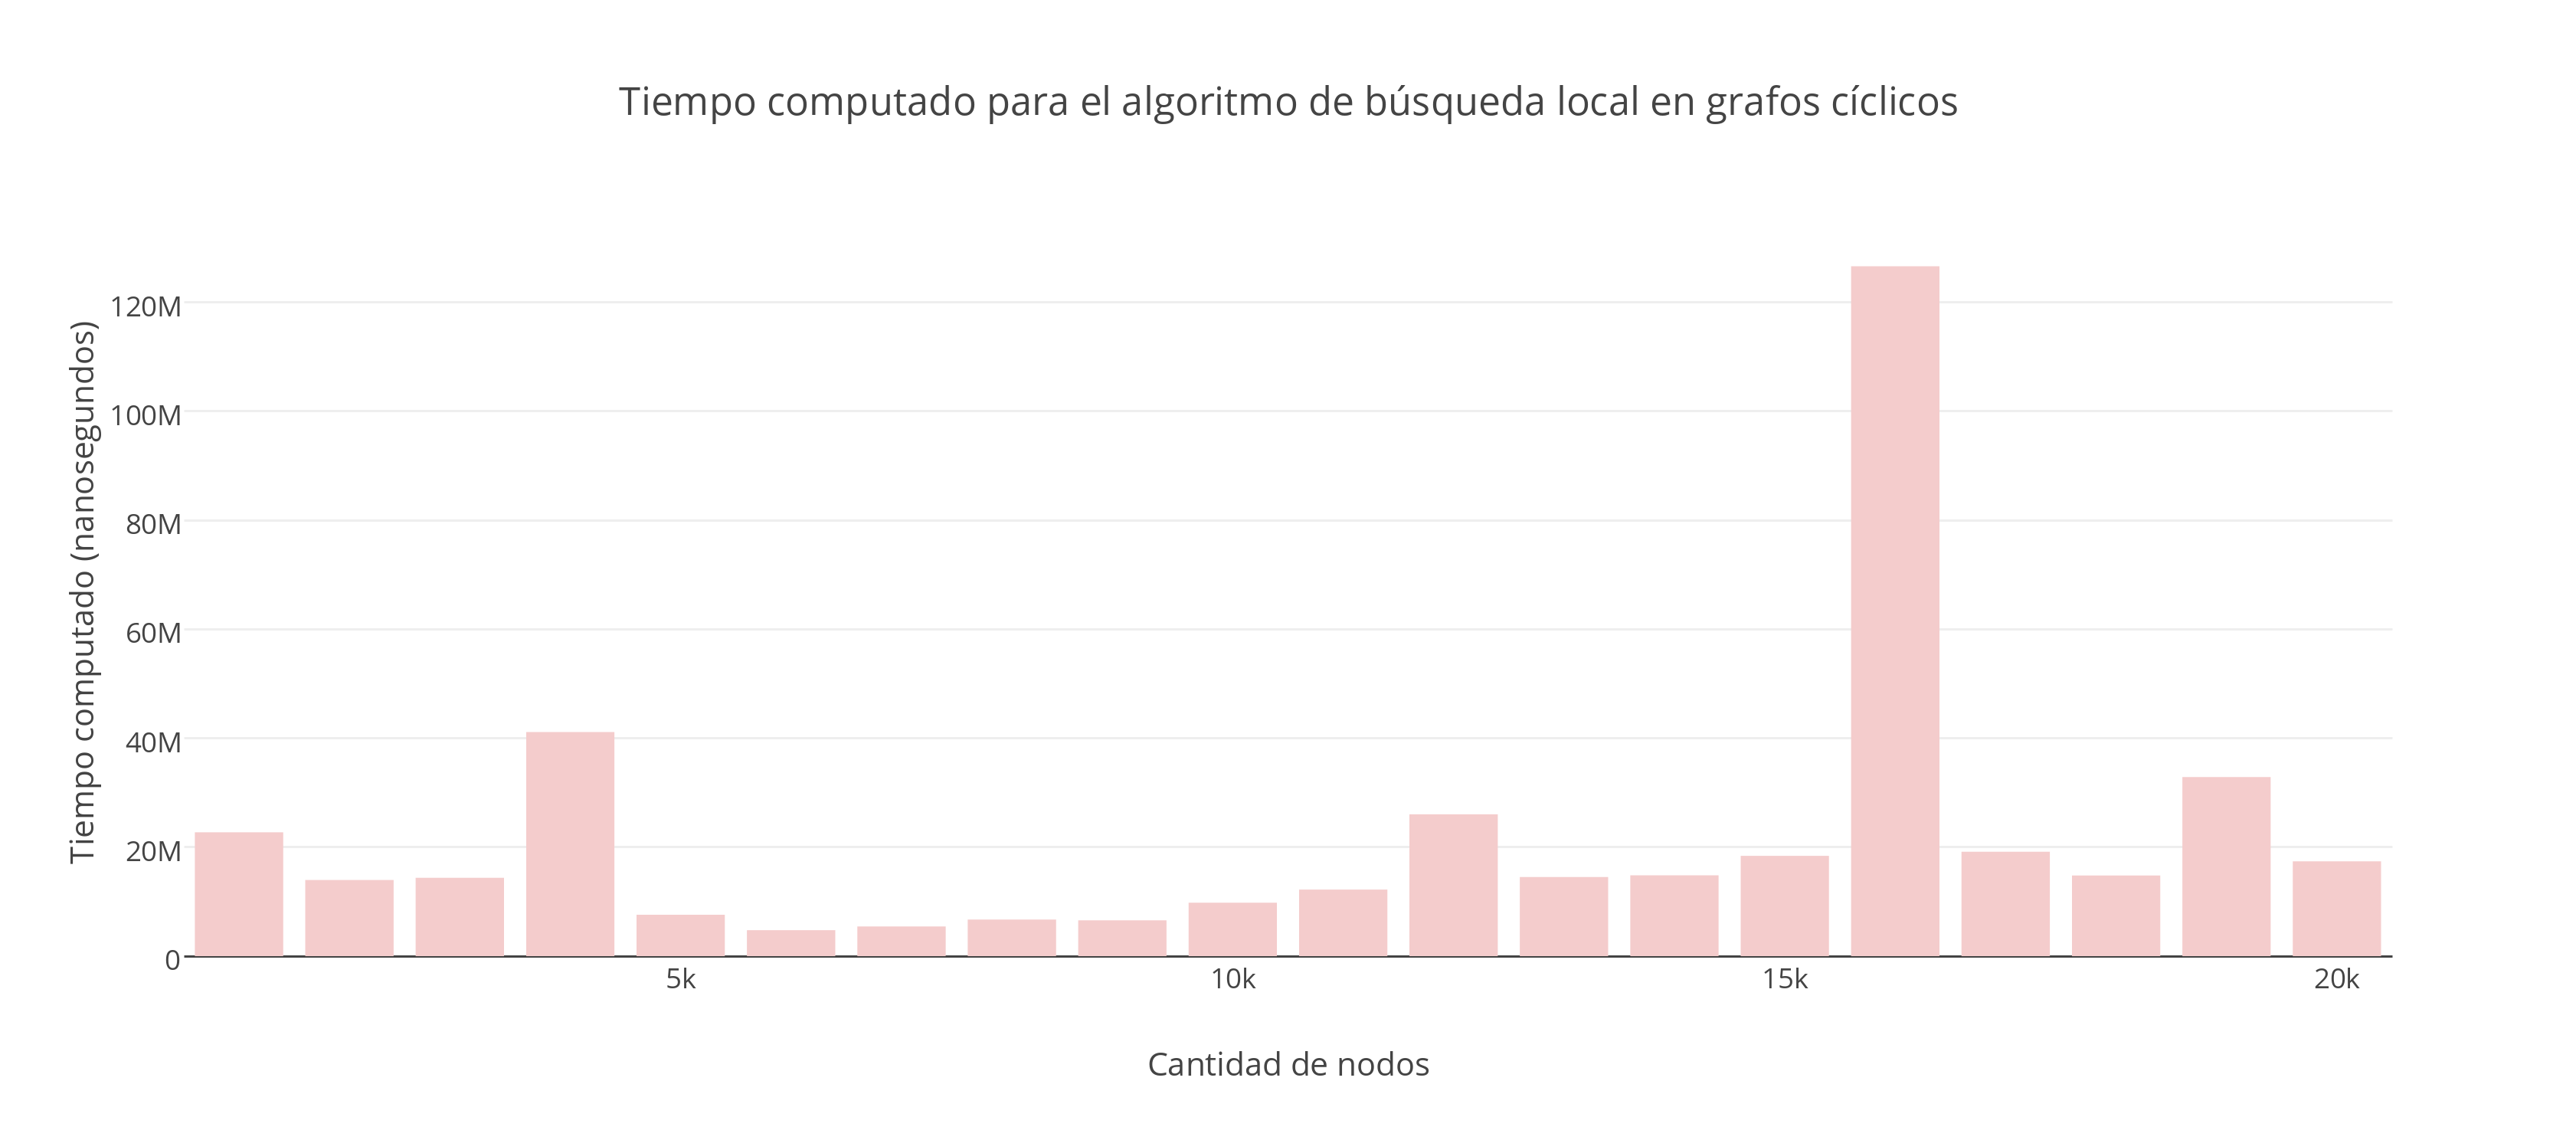
\includegraphics[width=18cm]{imagenes/Ej5/TiempoLocalCiclico.png}
 	\label{TiempoLocalCiclico}
    \end{center}
  \end{figure}

Esto se manifiesta en la figura \ref{ComparacionTiemposCiclico}. Allí graficamos el porcentaje de tiempo ejecución de cada algoritmo para cada instancia en función del tiempo total de cómputo.\\
La comparativa se realizó de esta manera debido a que no son algoritmos que corran sobre instancias iguales: El algoritmo de búsqueda local busca mejorar un resultado ya obtenido por el algoritmo goloso y recibe nodos que se asumen bien coloreados de acuerdo a algún criterio prefijado.

 \begin{figure}[H]
    \begin{center}
  	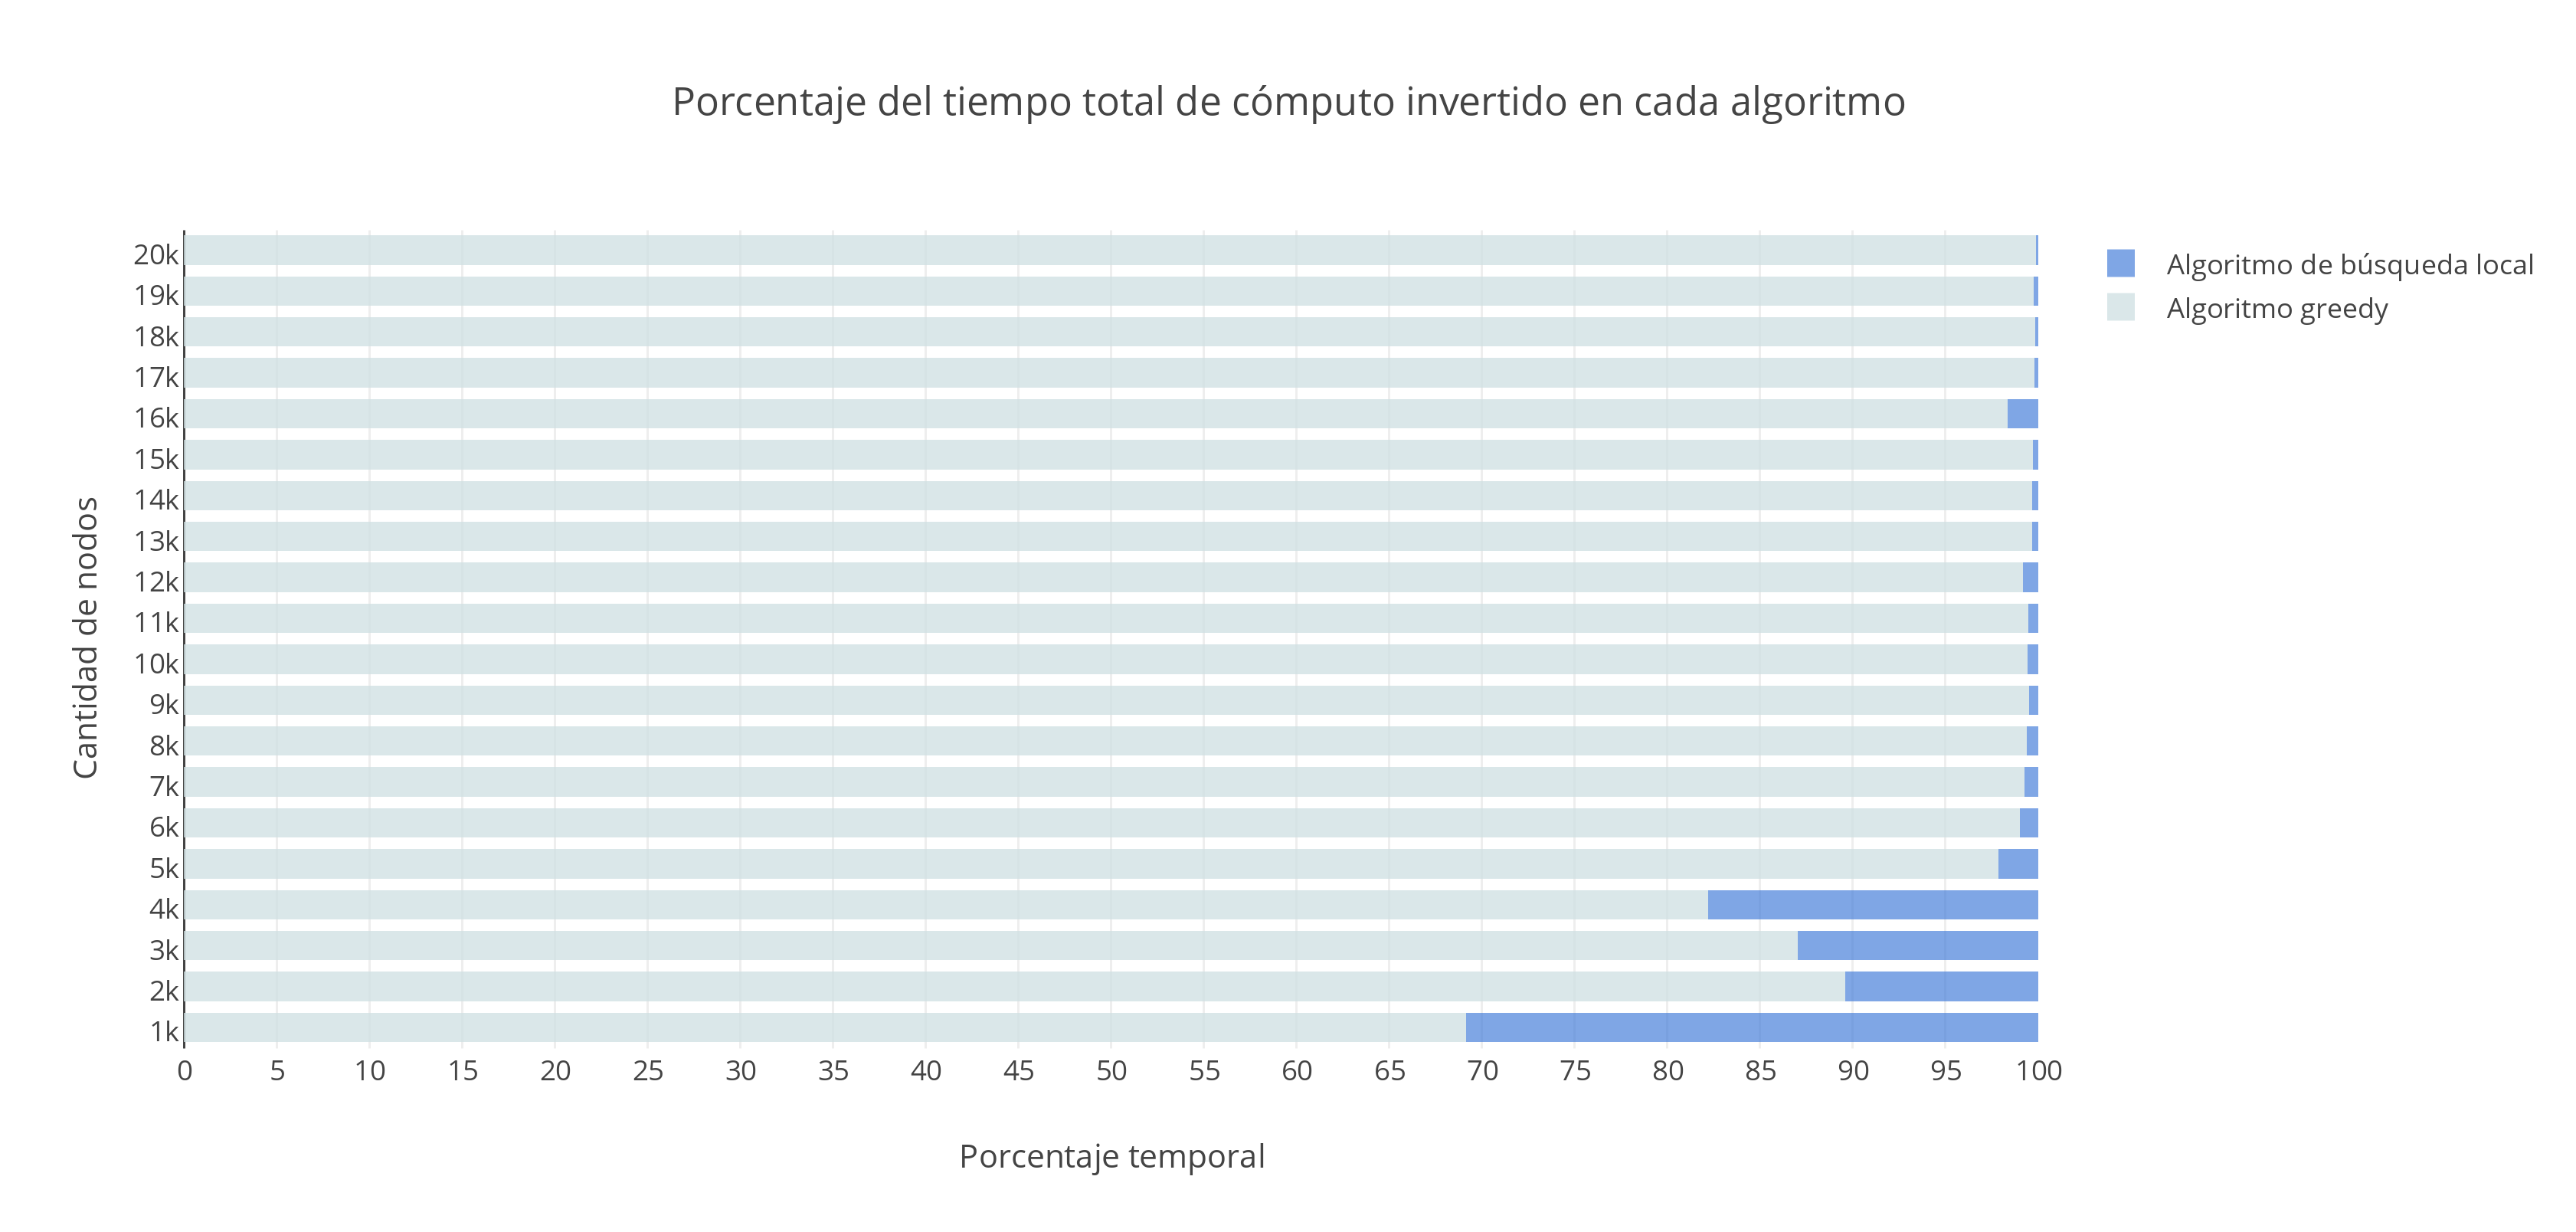
\includegraphics[width=18cm]{imagenes/Ej5/ComparacionTiemposCiclico.png}
 	\label{ComparacionTiemposCiclico}
    \end{center}
  \end{figure}

Por último, el gráfico \ref{ComparacionConflictosCiclico} nos muestra que la cantidad de conflictos entre el output de los distintos algoritmos no varía notoriamente. Esto nos fuerza a concluir que en situaciones en las que se anticipa que el grafo pueda llegar a tener una estructura similar a uno cíclico y no sea estrictamente necesario conseguir un coloreo tan óptimo como sea posible, puede ser conveniente tomar los resultados arrojados por el primer algoritmo.

 \begin{figure}[H]
    \begin{center}
  	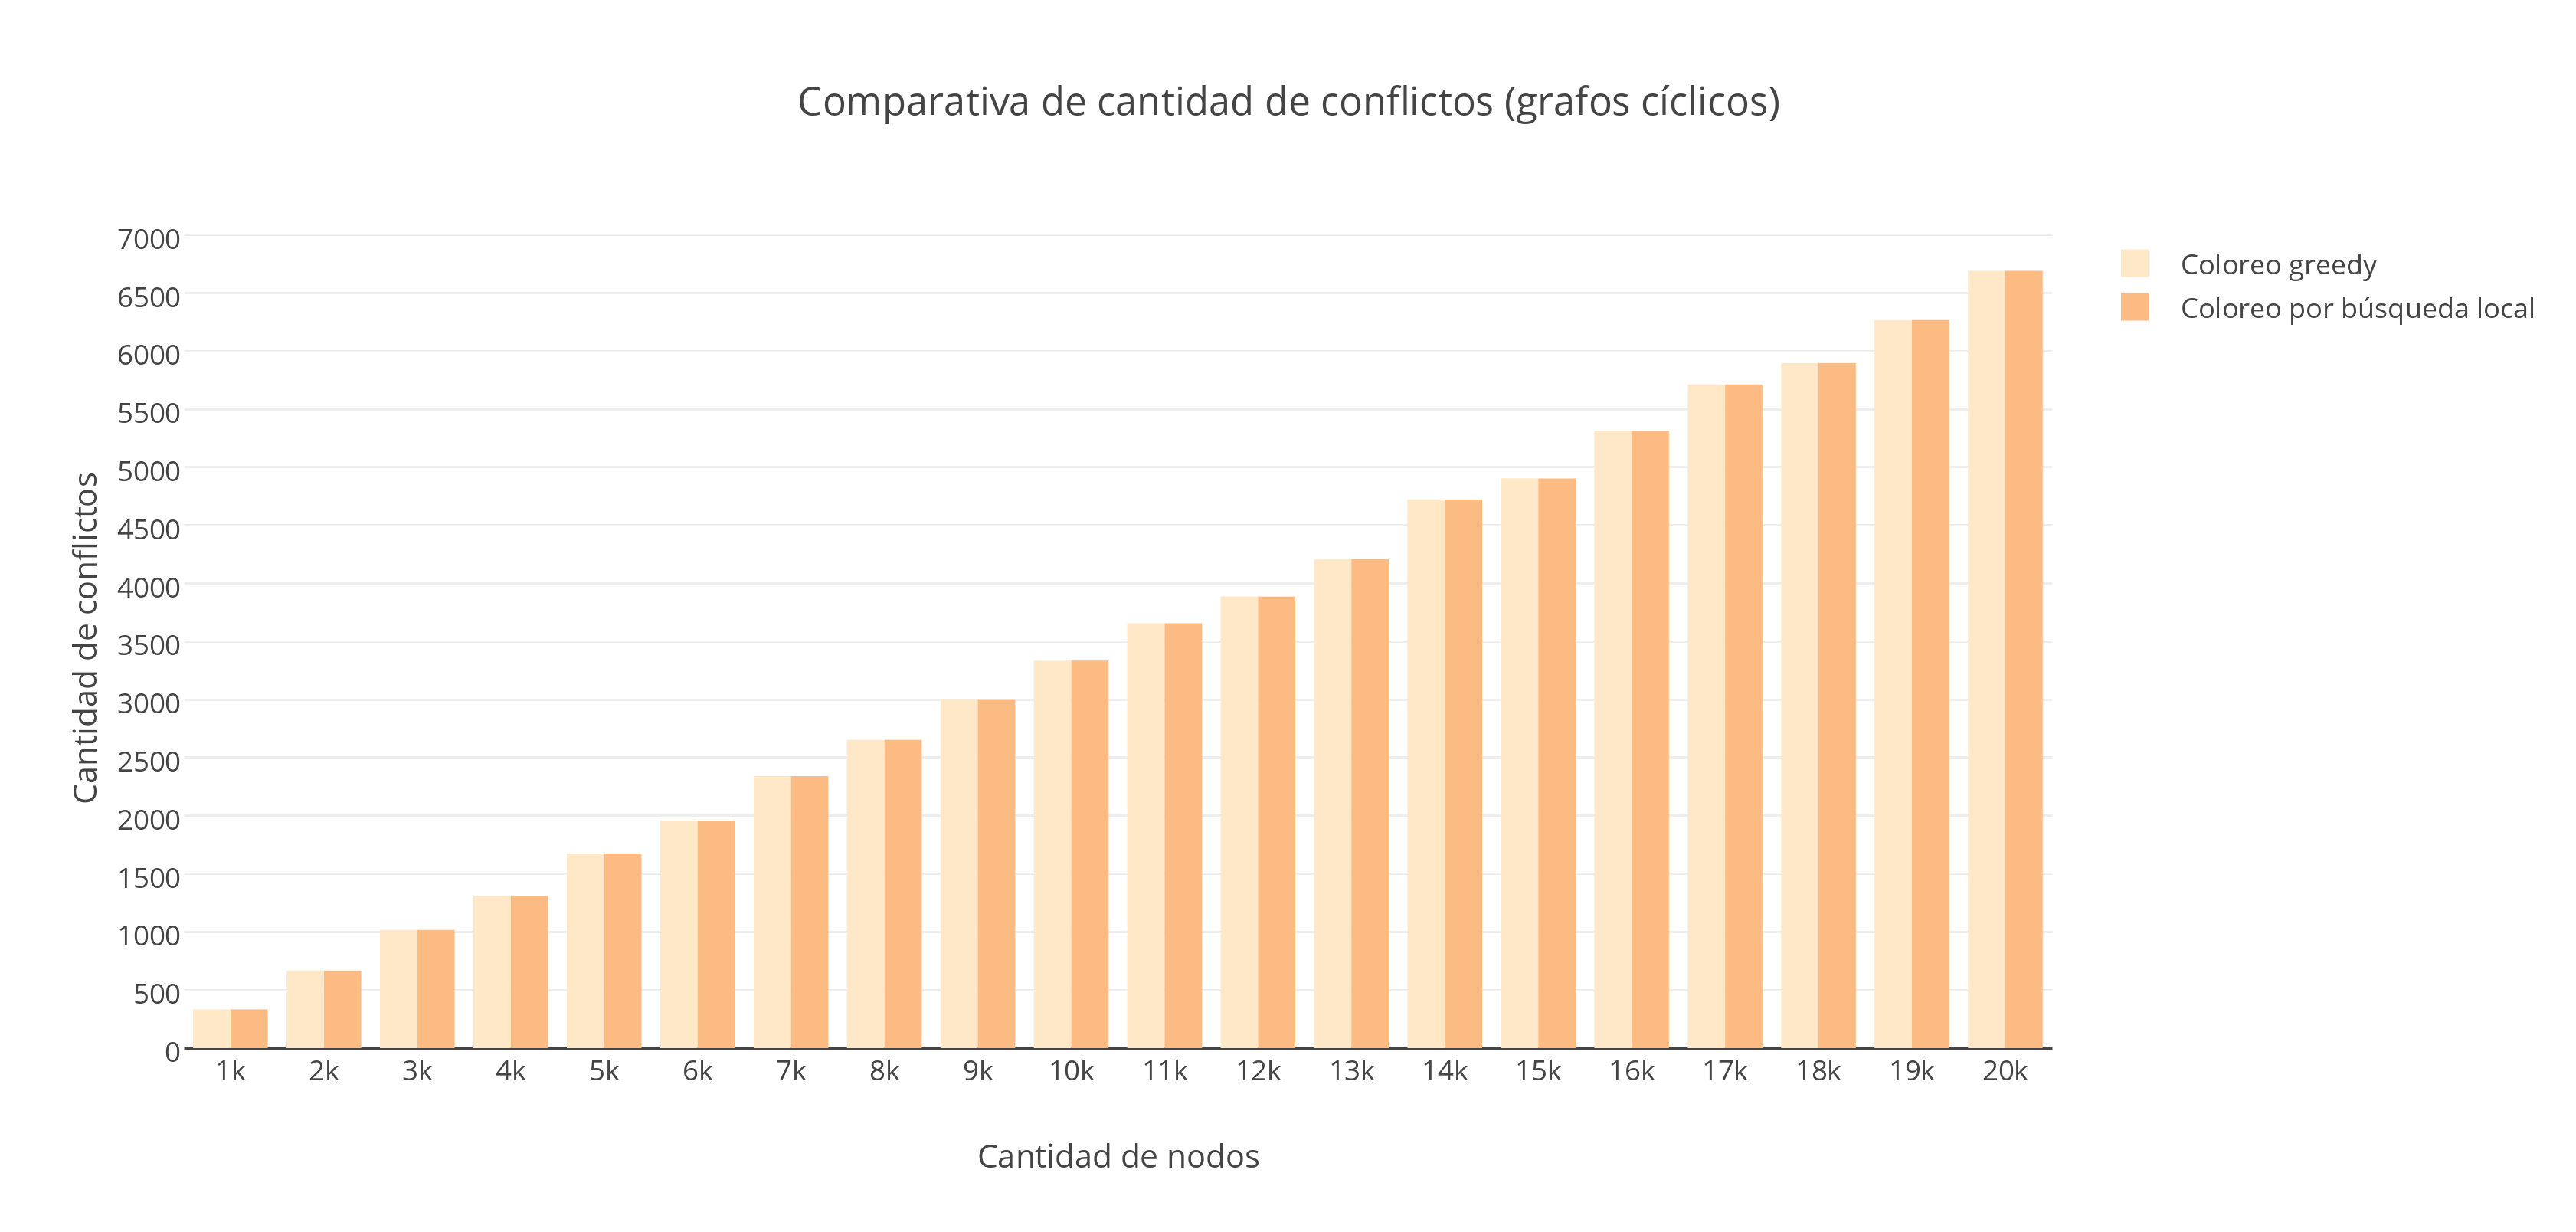
\includegraphics[width=18cm]{imagenes/Ej5/ComparacionConflictosCiclico.png}
 	\label{ComparacionConflictosCiclico}
    \end{center}
  \end{figure}


\subsection {Resultados obtenidos a partir de grafos completos} 

En las figuras \ref{TiempoGreedyCompleto} y \ref{TiemposLocalCompleto} muestran los tiempos (junto a sus cotas temporales) medidos observados para ambos algoritmos ejecutados sobre grafos completos de distintos tamaños.\\
Se hace realmente visible la direfencia en cuanto a costos temporales en la figura \ref{ComparacionTiemposCompleto}, en la cual se exhiben solapadas las barras que indican el tiempo de cómputo medido para cada algoritmo.

 \begin{figure}[H]
    \begin{center}
  	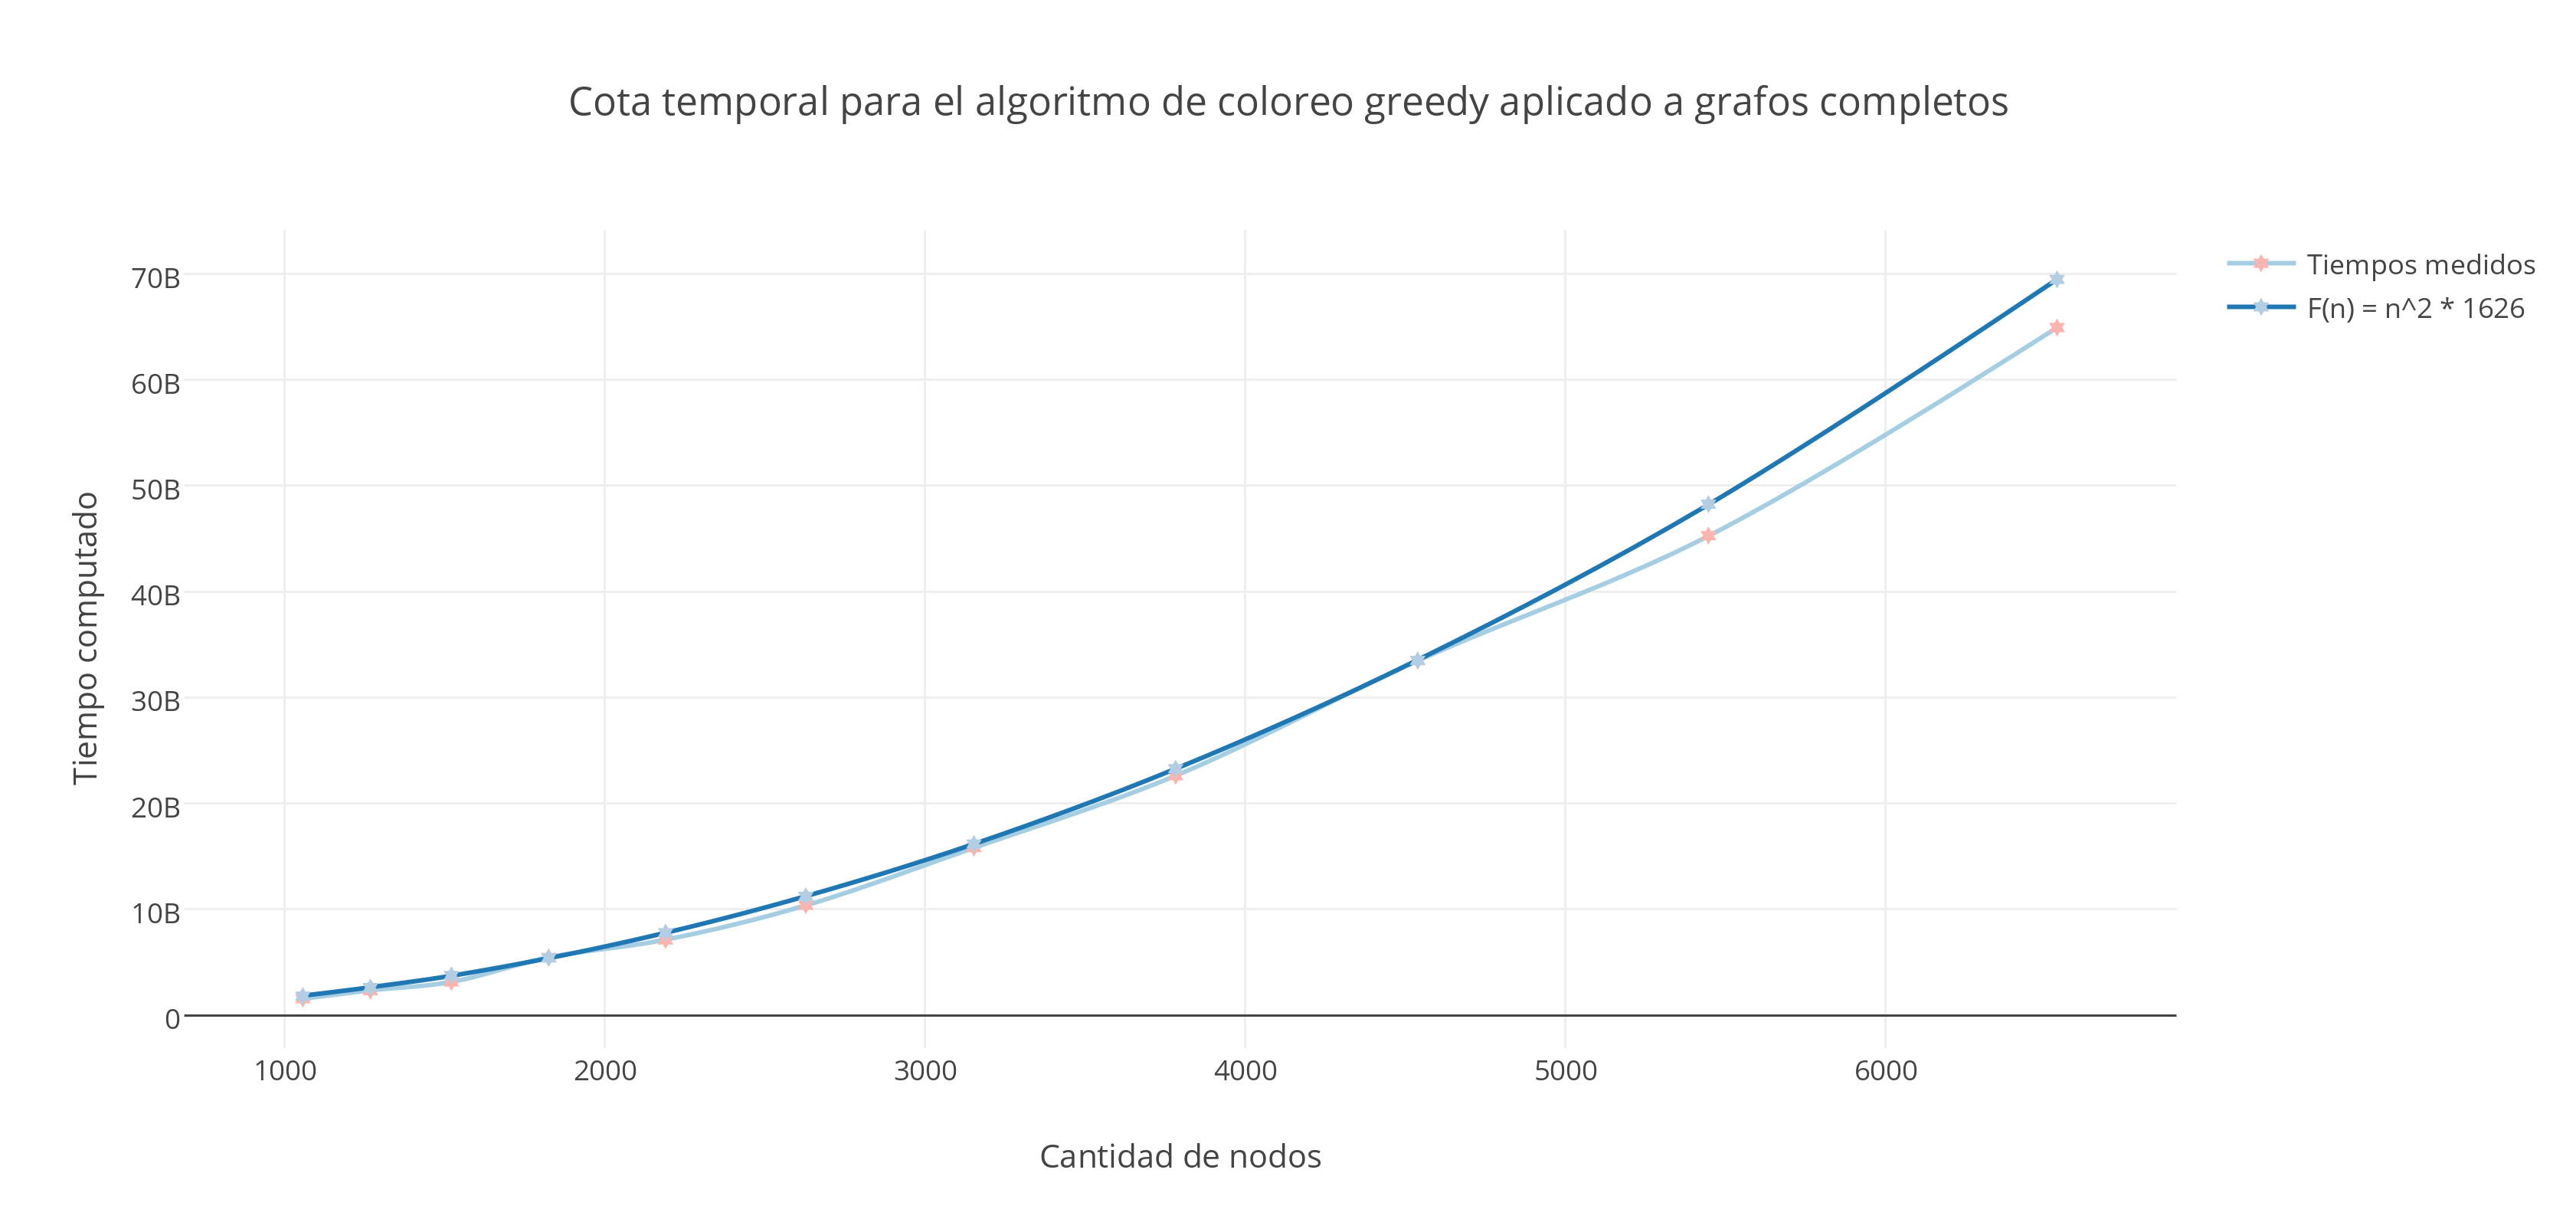
\includegraphics[width=18cm]{imagenes/Ej5/TiempoGreedyCompleto.png}
 	\label{TiempoGreedyCompleto}
    \end{center}
  \end{figure}

 \begin{figure}[H]
    \begin{center}
  	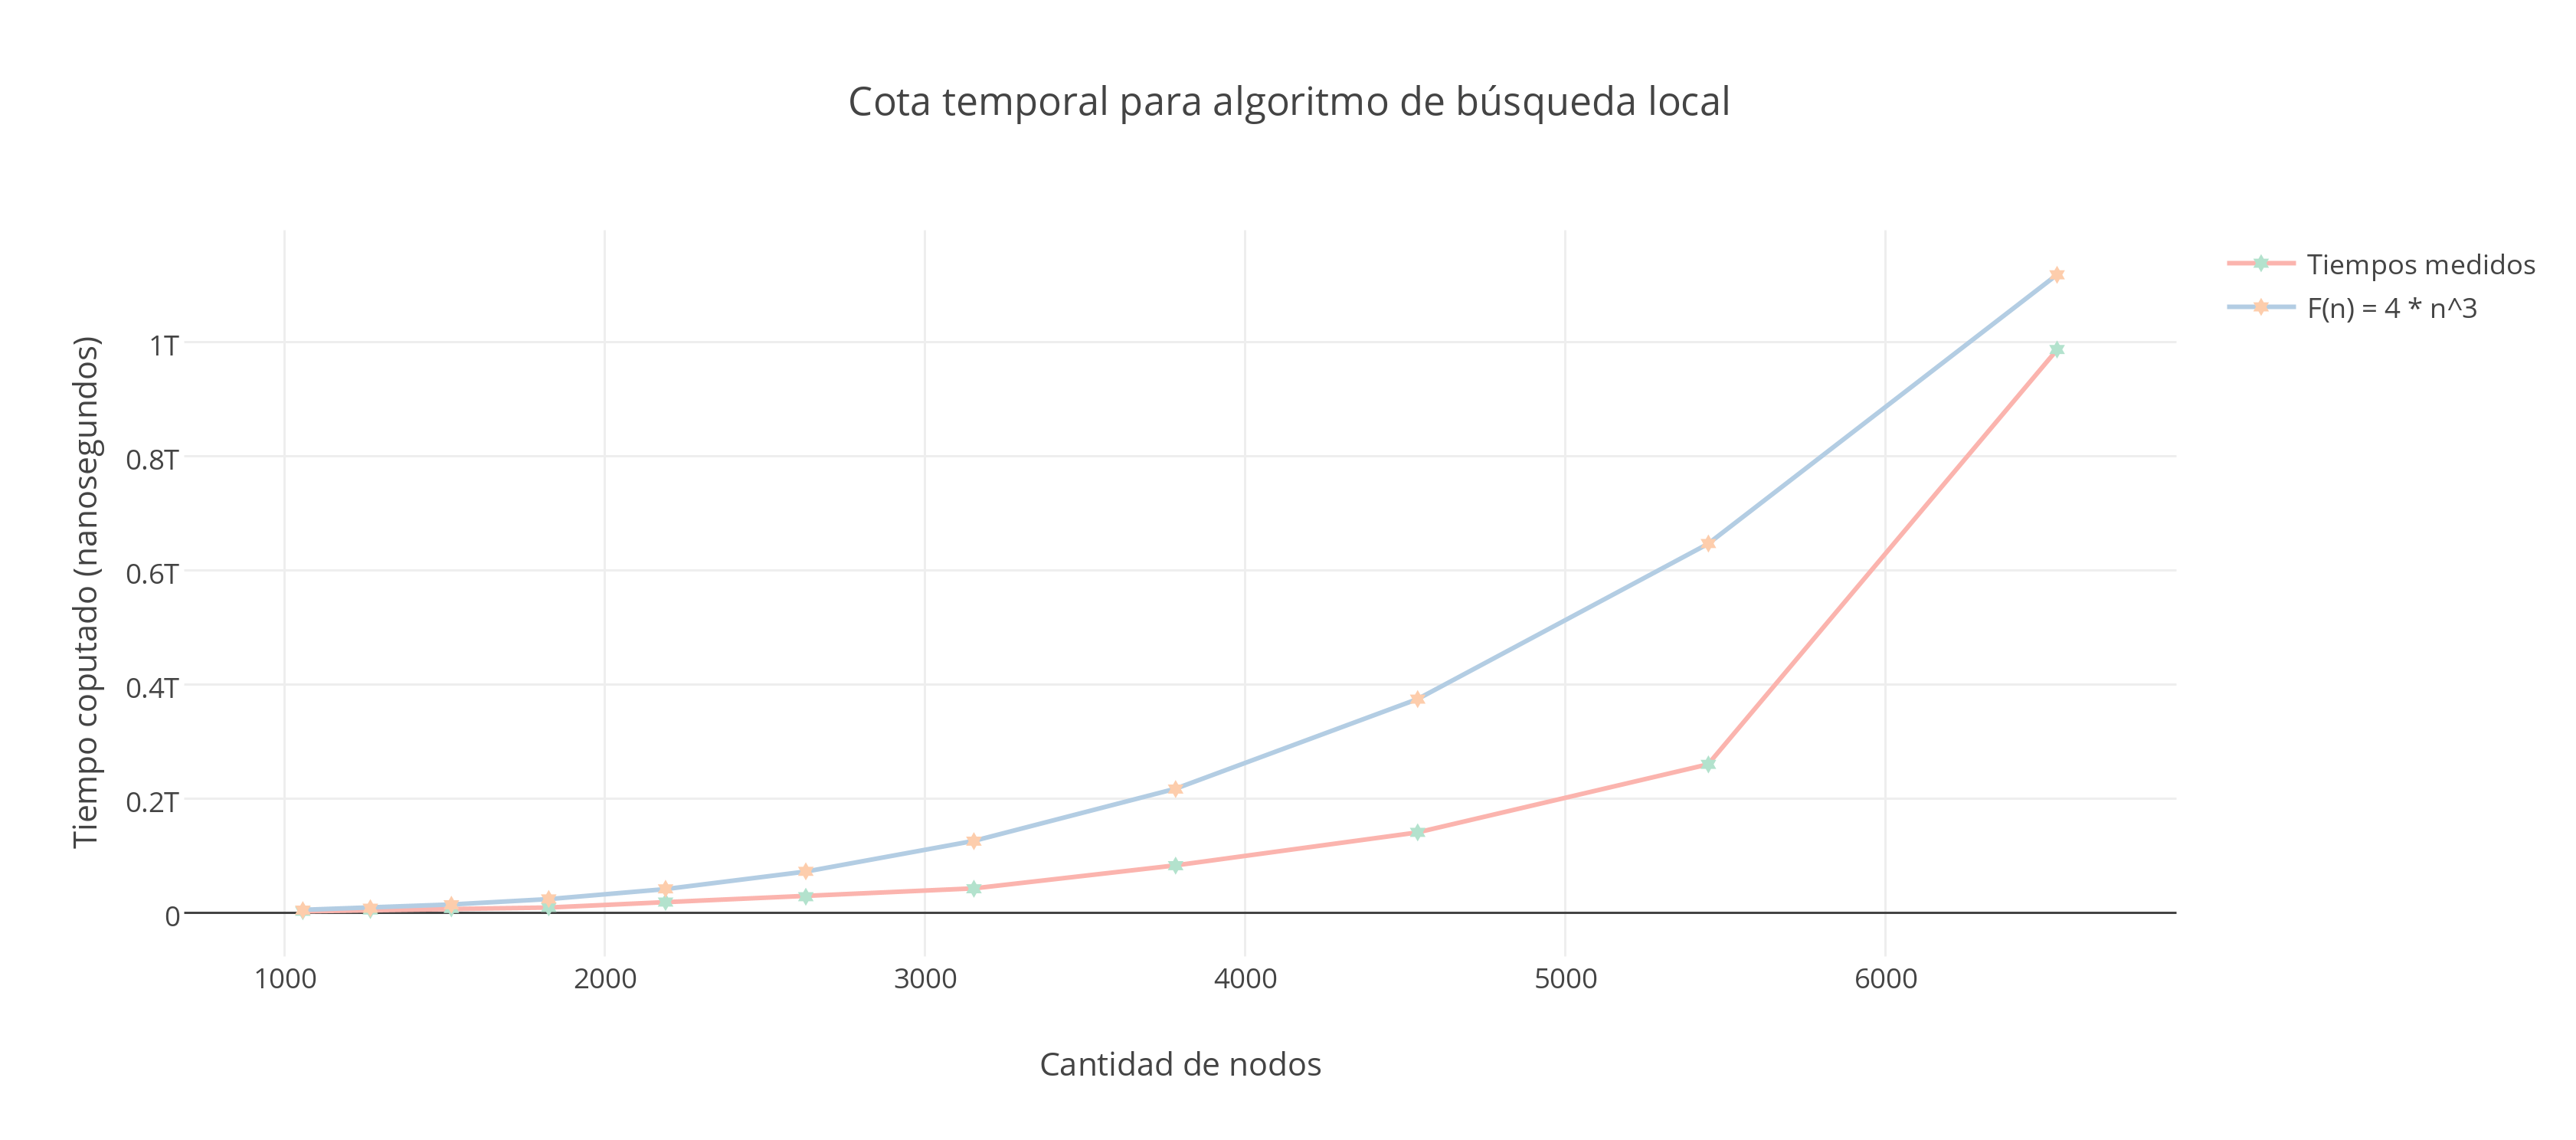
\includegraphics[width=18cm]{imagenes/Ej5/TiemposLocalCompleto.png}
 	\label{TiemposLocalCompleto}
    \end{center}
  \end{figure}

 \begin{figure}[H]
    \begin{center}
  	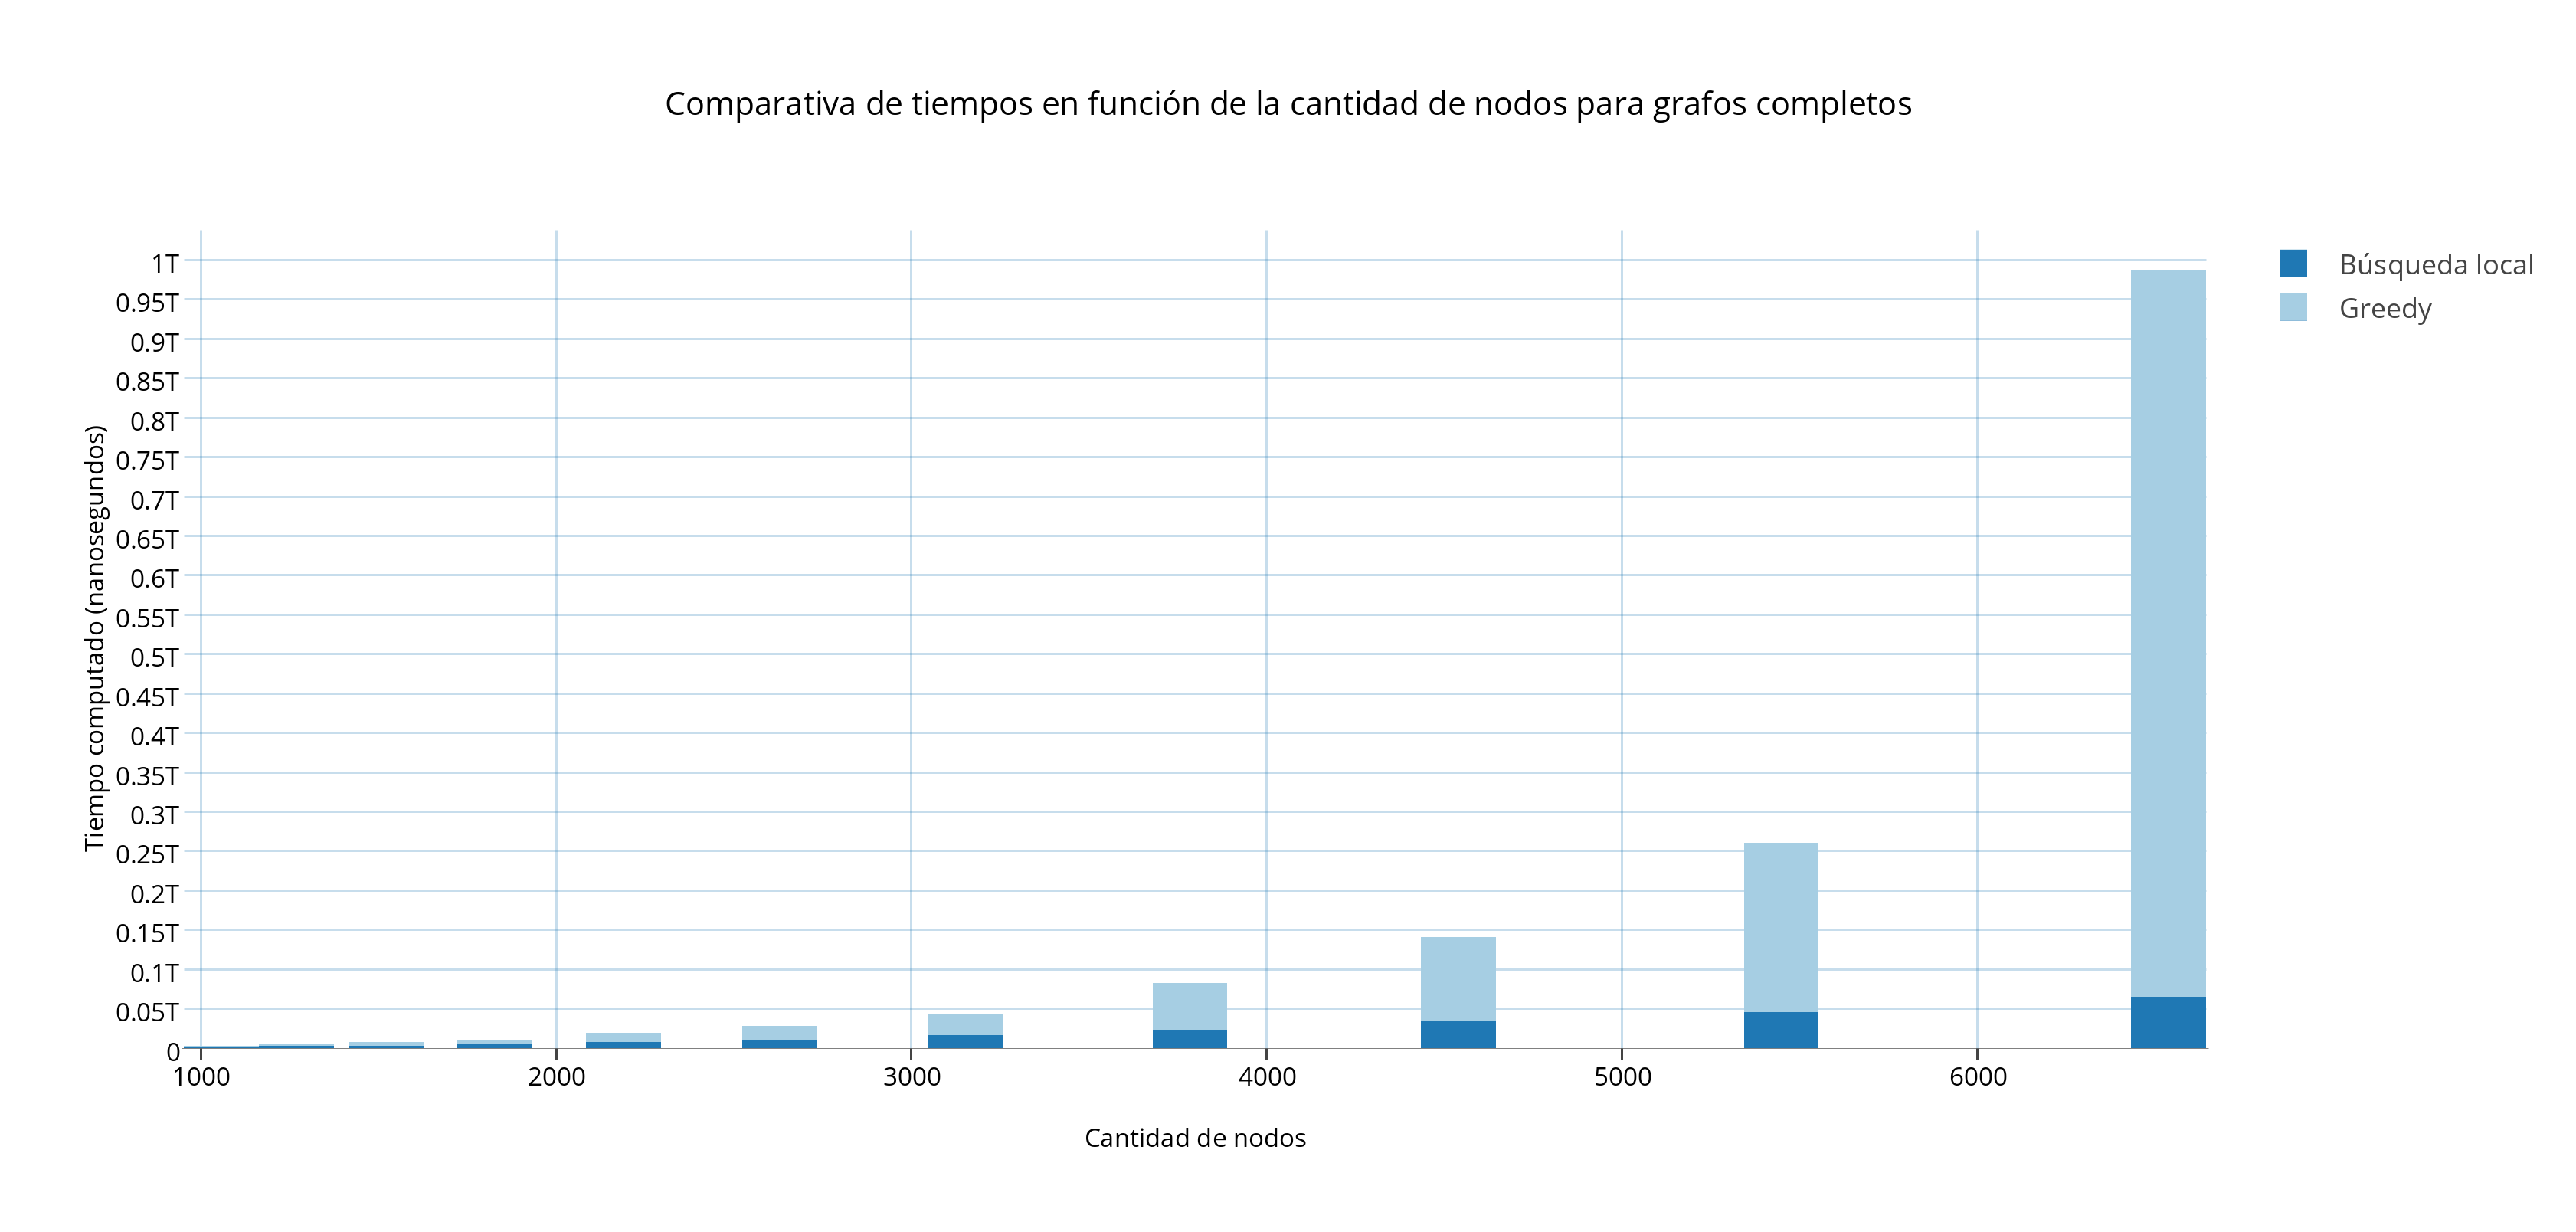
\includegraphics[width=18cm]{imagenes/Ej5/ComparacionTiemposCompleto.png}
 	\label{ComparacionTiemposCompleto}
    \end{center}
  \end{figure}

Sin embargo, a diferencia de lo observado en la figura \ref{ComparacionConflictosCiclico}, en la ilustración \ref{ComparacionConflictosCompleto} puede apreciarse la disminución en la cantidad de conflictos resultante del posprocesamiento del grafo obtenido luego de la ejeución del algoritmo goloso.\\
Dicho esto, pareciera ser que en los casos en que el grafo no es esparso, el algoritmo de búsqueda local si es una buena opción en términos del costo temporal y el beneficio cualitativo del resultado.

 \begin{figure}[H]
    \begin{center}
  	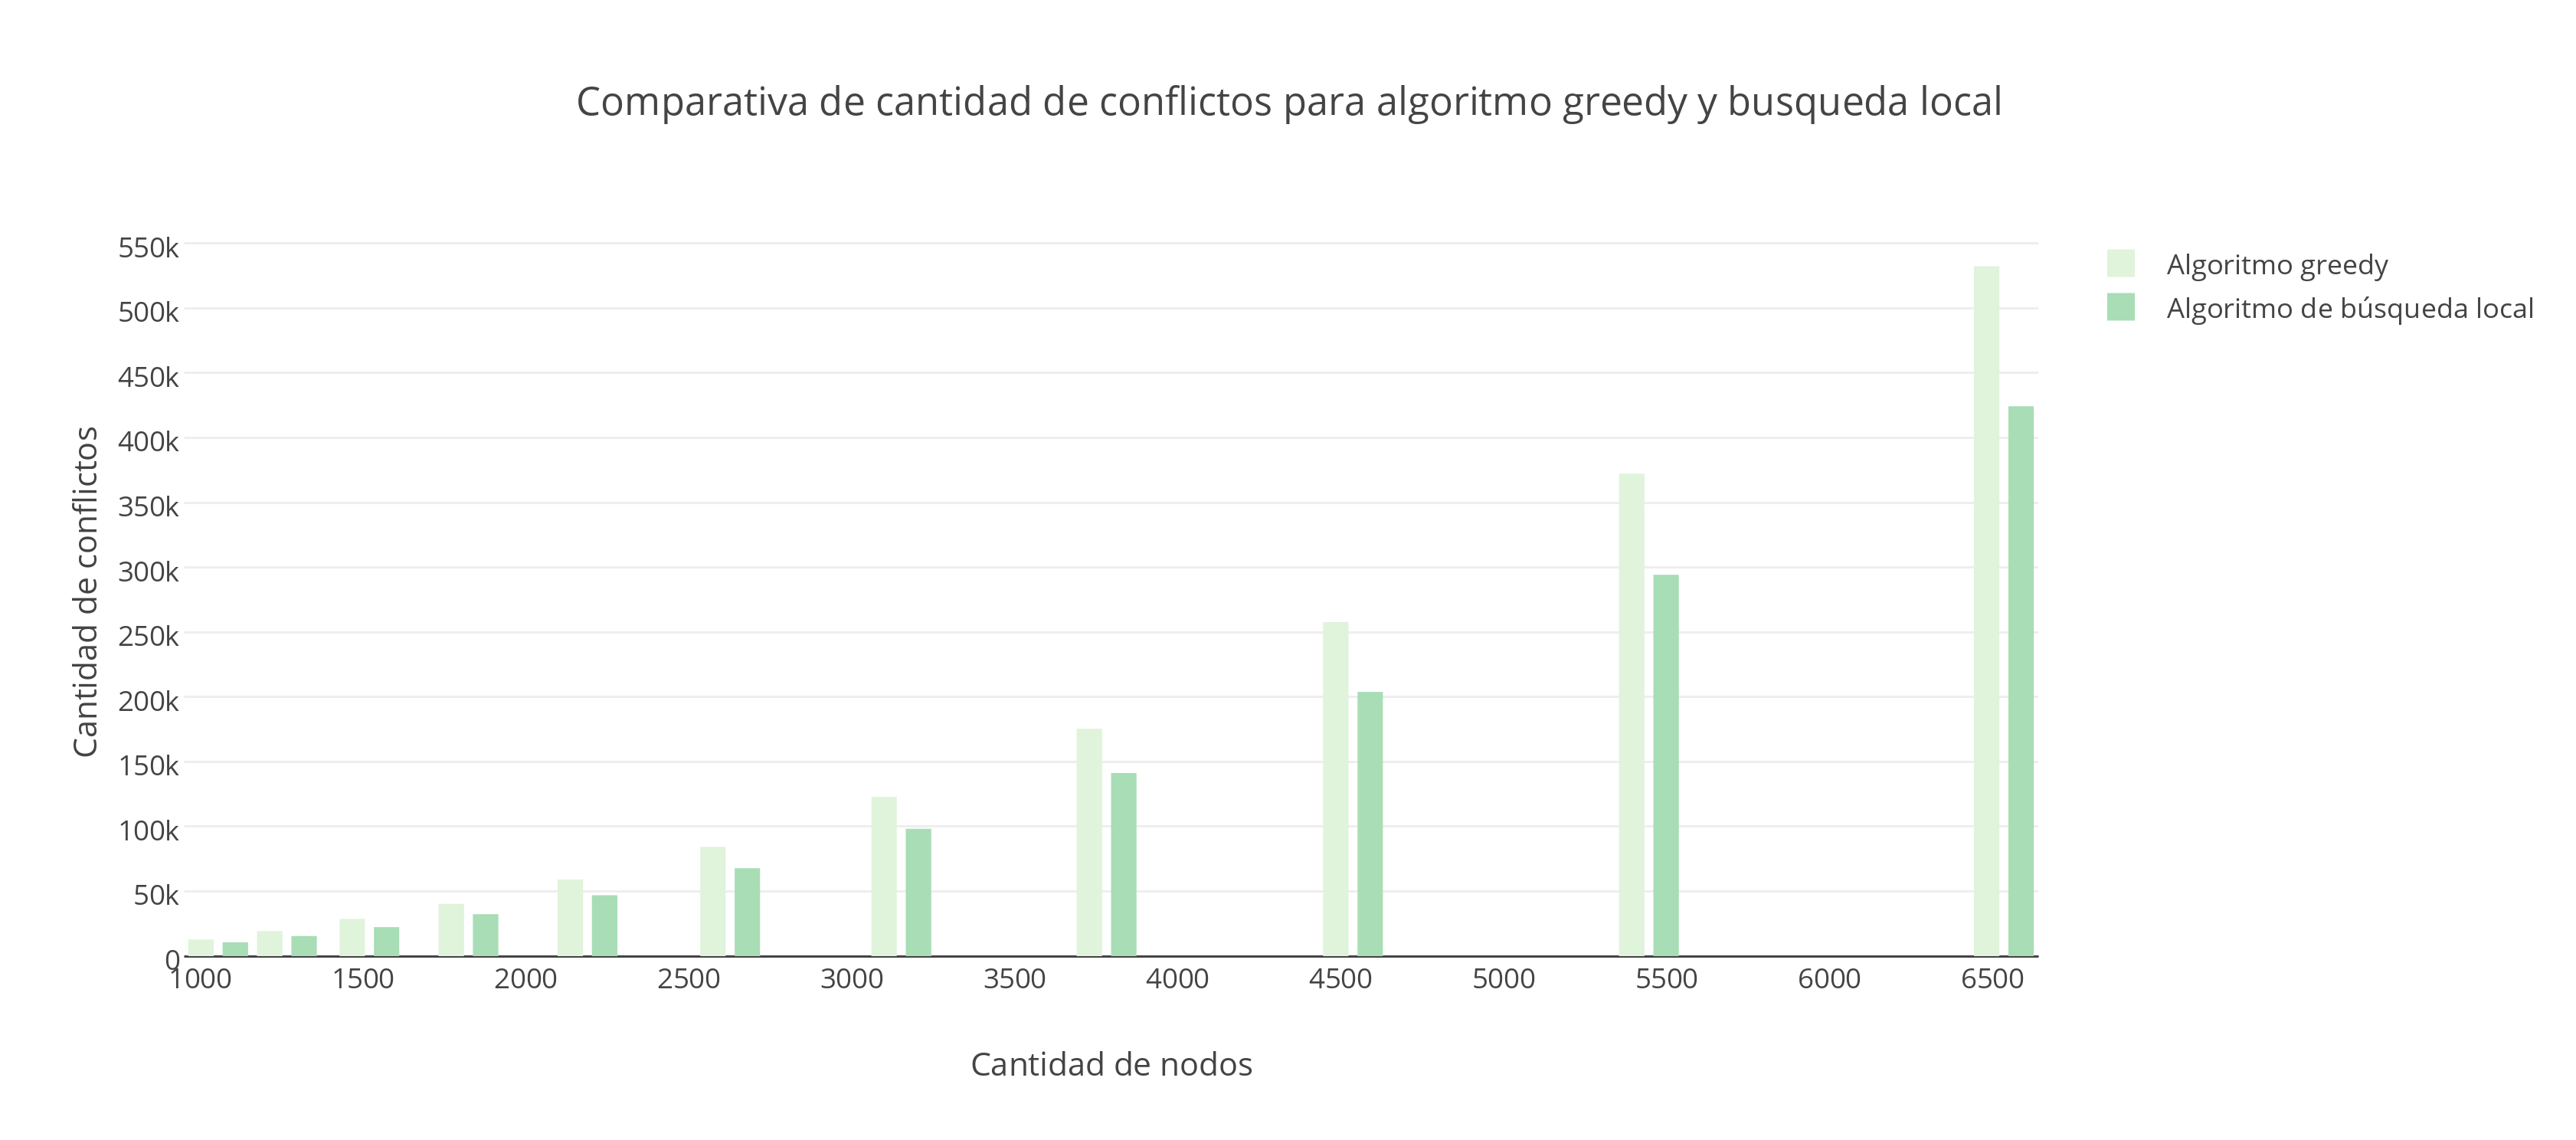
\includegraphics[width=18cm]{imagenes/Ej5/ComparacionConflictosCompleto.png}
 	\label{ComparacionConflictosCompleto}
    \end{center}
  \end{figure}

\subsection {Resultados obtenidos a parir de grafos bipartitos completos} 

\textcolor{red}{\huge{AGREGAR TODOS LOS GRAFICOS QUE ESTAN EN LA CARPETA IMAGENES/EJ5/BIPARTITOS Y COMENTARLOS}}